\section{Results}
\label{sec:results}

\begin{table}[t]
\centering
\caption{Accuracy (\%) and \rougel by shot count $K$, pooled over all demonstration sets and orders. $K=0$ is zero-shot. Majority-class accuracy is about 50 (\sst, \rte) and 33 (\mnli). Best per column in \textbf{bold}.}
\label{tab:accuracy}
\resizebox{\textwidth}{!}{%
\begin{tabular}{@{}lcccccccccccccccc@{}}
\toprule
 & \multicolumn{4}{c}{\sst (acc)} & \multicolumn{4}{c}{\rte (acc)} & \multicolumn{4}{c}{\mnli (acc)} & \multicolumn{4}{c}{\samsum (\rougel)} \\
\cmidrule(lr){2-5} \cmidrule(lr){6-9} \cmidrule(lr){10-13} \cmidrule(lr){14-17}
Model & $K$=0 & 1 & 4 & 8 & 0 & 1 & 4 & 8 & 0 & 1 & 4 & 8 & 0 & 1 & 4 & 6 \\
\midrule
0.5B & 89.5 & 86.8 & 90.1 & 90.8 & 60.5 & 57.6 & 69.0 & 69.6 & 48.0 & 46.2 & 54.7 & 57.0 & 19.9 & 24.8 & 20.9 & 21.8 \\
1.5B & 92.5 & 93.5 & 93.5 & 93.9 & 77.5 & 77.8 & 82.6 & 83.1 & 64.0 & 64.6 & 65.5 & 66.1 & 27.3 & 32.0 & 34.8 & 34.9 \\
3B   & 90.0 & 92.4 & 93.2 & 93.3 & 84.5 & 82.6 & 84.9 & 85.0 & 74.0 & 78.9 & 81.3 & 81.4 & 27.0 & 32.2 & 33.7 & 34.1 \\
7B   & 91.5 & \textbf{93.6} & 93.3 & 93.4 & 88.0 & 84.5 & 86.1 & 85.7 & \textbf{81.0} & \textbf{83.3} & \textbf{83.3} & \textbf{84.0} & \textbf{33.5} & 36.0 & 36.0 & 37.5 \\
14B  & \textbf{94.0} & \textbf{93.6} & \textbf{94.4} & \textbf{94.4} & \textbf{88.5} & \textbf{89.6} & \textbf{91.1} & \textbf{91.2} & 80.0 & 79.0 & 77.8 & 82.5 & 31.9 & \textbf{37.6} & \textbf{38.4} & \textbf{38.6} \\
\bottomrule
\end{tabular}}
\end{table}


\para{Demonstrations help small models most.}
\Tabref{tab:accuracy} gives the accuracy context for all later results.
All models are well above the majority class.
Demonstrations add the most for small models (0.5B on \rte: 60.5 zero-shot \vsx 69.6 at $K=8$) and little for large ones (14B on \sst: 94.0 \vsx 94.4).
On \mnli, 14B accuracy \emph{drops} below zero-shot at $K=4$ (77.8 \vsx 80.0) and recovers at $K=8$ (82.5), so a few unbalanced demonstrations can hurt a strong model.

\subsection{H1: order variance is flat from two shots on}
\label{sec:h1}

\begin{figure}[t]
\centering
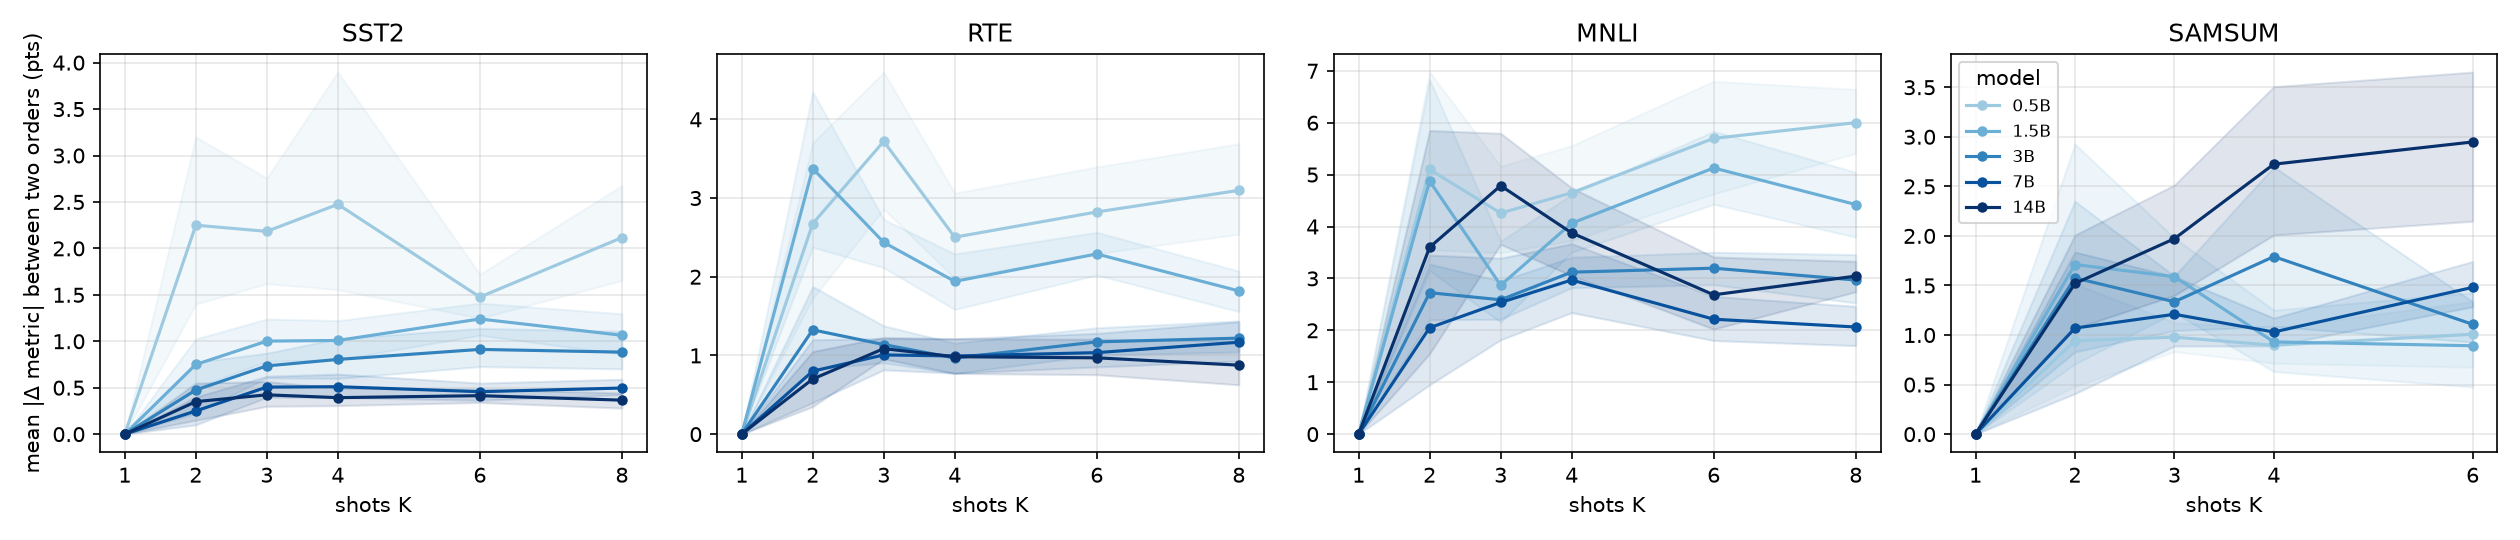
\includegraphics[width=0.95\linewidth]{figures/fig1_pairgap_vs_K.png}
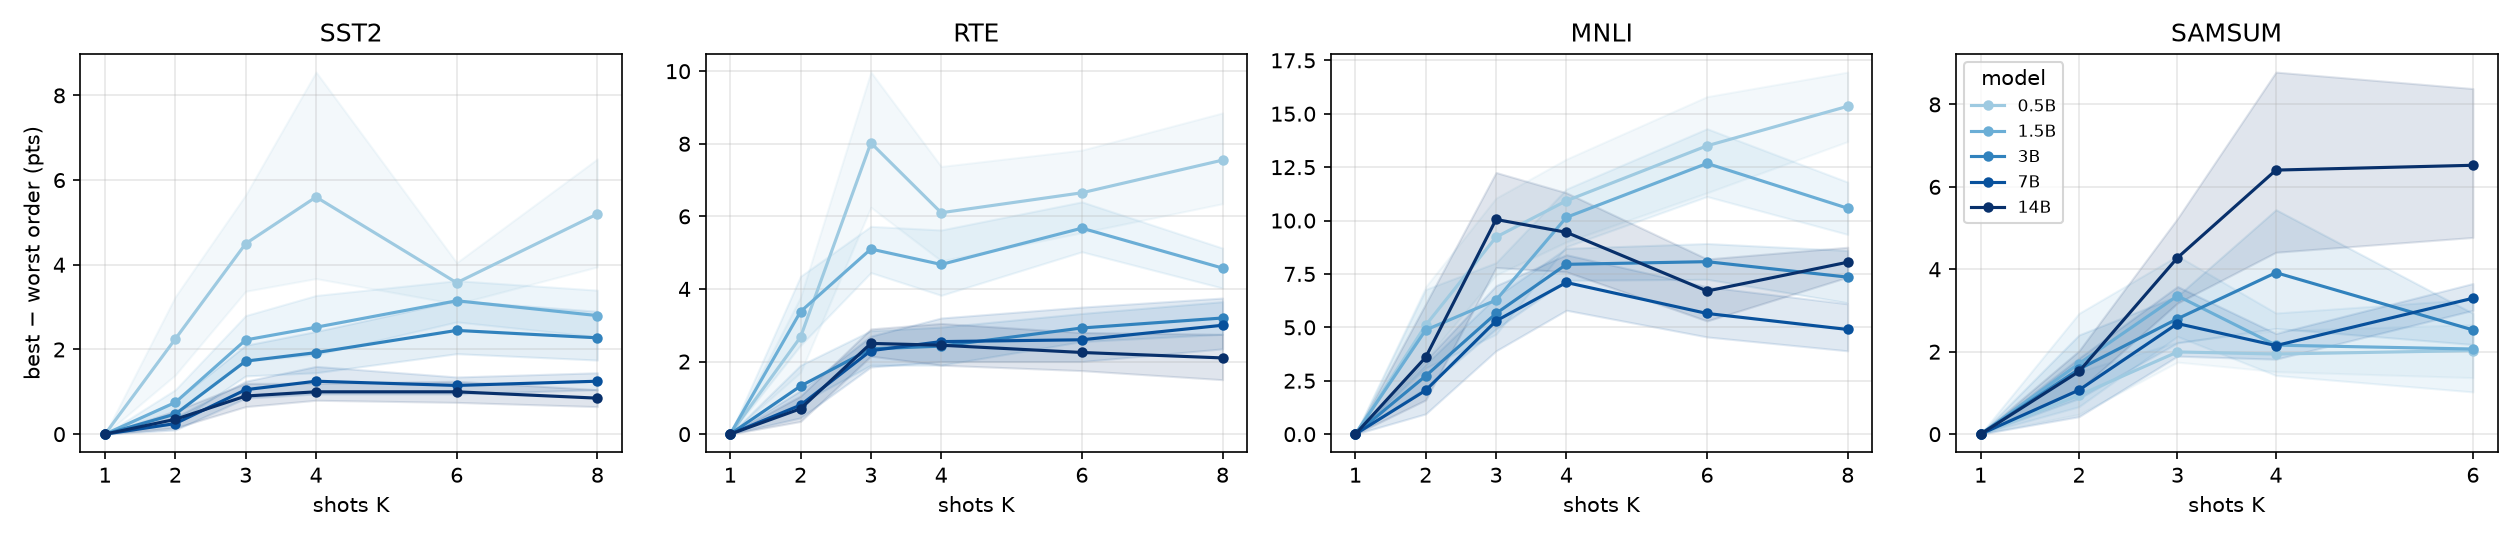
\includegraphics[width=0.95\linewidth]{figures/fig2_range_vs_K.png}
\caption{Order sensitivity \vsx shot count $K$ for each task and model (shaded: 95\% bootstrap CI over demonstration sets). \figtop Mean pairwise gap (\pgap), whose expectation does not depend on the number of orders sampled: from $K=2$ the curves are roughly flat. \figbottom Best--worst range over the sampled orders: it shows a ``rise until $K=3$--4, then plateau'' shape, which tracks the number of available orders (2 at $K=2$, 6 at $K=3$, 8 for $K\geq4$) rather than the model.}
\label{fig:h1}
\end{figure}

\begin{table}[t]
\centering
\caption{H1: mean pairwise order gap (\pgap, points) by shot count, pooled over models, with Spearman correlations between $K$ and the gap for $K\leq4$ and $K\geq4$. $K=1$ has a single order and zero variance by construction. From $K=2$ the gap is essentially flat.}
\label{tab:h1}
\small
\begin{tabular}{@{}lccccccc@{}}
\toprule
Task & $K$=2 & 3 & 4 & 6 & 8 & $\rho$ ($K\leq4$) [$p$] & $\rho$ ($K\geq4$) [$p$] \\
\midrule
\sst & 0.94 & 1.10 & 1.19 & 1.02 & 1.12 & 0.17 [0.007] & 0.03 [0.63] \\
\rte & 2.03 & 2.09 & 1.60 & 1.82 & 1.79 & $-$0.02 [0.71] & 0.07 [0.26] \\
\mnli & 3.88 & 3.34 & 3.81 & 4.12 & 3.99 & 0.16 [0.016] & $-$0.02 [0.78] \\
\samsum (\rougel) & 1.36 & 1.42 & 1.47 & 1.49 & -- & 0.09 [0.40] & 0.07 [0.61] \\
\bottomrule
\end{tabular}
\end{table}


{\bf Does order variance rise until 4 shots and then plateau?}
\Tabref{tab:h1} and \figref{fig:h1} (top) show that it does not.
Measured with \pgap, order variance is already at its plateau at $K=2$.
Over $K=2$--4 there is a weak upward trend on \sst and \mnli ($\rho\approx0.16$--$0.17$, $p<0.02$), but the $K$-means differ by less than 0.5 points; \rte and \samsum show no trend.
Per model, only 1 of 20 task--model curves rises significantly over $K=2$--4 (\sst, 3B).
For $K\geq4$, 3 of 20 curves have a significant trend, with mixed signs (\mnli 0.5B up, \mnli 7B down, \samsum 7B up).

The best--worst range, in contrast, shows exactly the hypothesized shape (\figref{fig:h1}, bottom): on \mnli, for instance, the 0.5B range climbs from about 5 points at $K=2$ to about 11 at $K=4$.
This shape follows the number of orders we can sample (2, then 6, then 8), because the maximum minus the minimum of more draws is larger.
{\bf H1 is not supported}; the apparent support is a measurement artifact.
Studies that compare ranges over all $K!$ orders, or over a fixed small number of permutations, across shot counts should be read with this in mind.

\subsection{H4: NLI is more order-sensitive than sentiment, but the thresholds fail}
\label{sec:h4}

\begin{table}[t]
\centering
\caption{H4: order sensitivity at $K\geq4$ (8 orders per demonstration set; 6 for \samsum). ``Mean range'' averages best--worst over demonstration sets; ``max range'' is the worst single set. Units are accuracy points (\rougel points for \samsum). Lowest (least order-sensitive) per row in \textbf{bold}. Only the worst \mnli sets for 0.5B and 1.5B exceed 15 points.}
\label{tab:h4}
\small
\begin{tabular}{@{}llccccc@{}}
\toprule
Task & Statistic & 0.5B & 1.5B & 3B & 7B & 14B \\
\midrule
\multirow{4}{*}{\mnli} & mean range & 13.3 & 11.1 & 7.8 & \textbf{5.9} & 8.1 \\
 & max range & 21.7 & 17.5 & 11.7 & \textbf{9.8} & 11.7 \\
 & SD & 4.7 & 4.0 & 2.7 & \textbf{2.1} & 2.8 \\
 & \pgap & 5.5 & 4.5 & 3.1 & \textbf{2.4} & 3.2 \\
\midrule
\multirow{4}{*}{\rte} & mean range & 6.8 & 5.0 & 2.9 & 2.7 & \textbf{2.3} \\
 & max range & 12.5 & 8.5 & 5.2 & 5.2 & \textbf{4.0} \\
 & SD & 2.4 & 1.7 & 1.0 & 0.9 & \textbf{0.8} \\
 & \pgap & 2.8 & 2.0 & 1.1 & 1.1 & \textbf{0.9} \\
\midrule
\multirow{4}{*}{\sst} & mean range & 4.8 & 2.8 & 2.2 & 1.2 & \textbf{1.0} \\
 & max range & 15.5 & 6.7 & 6.0 & 2.0 & \textbf{1.5} \\
 & SD & 1.8 & 1.0 & 0.8 & \textbf{0.4} & \textbf{0.4} \\
 & \pgap & 2.0 & 1.1 & 0.9 & 0.5 & \textbf{0.4} \\
\midrule
\multirow{4}{*}{\samsum} & mean range & \textbf{2.0} & 2.1 & 3.2 & 2.7 & 6.5 \\
 & max range & \textbf{3.1} & 4.2 & 5.3 & 3.3 & 10.9 \\
 & SD & \textbf{0.8} & \textbf{0.8} & 1.2 & 1.1 & 2.4 \\
 & \pgap & 1.0 & \textbf{0.9} & 1.5 & 1.3 & 2.8 \\
\bottomrule
\end{tabular}
\end{table}


\Tabref{tab:h4} reports sensitivity at $K\geq4$, where every demonstration set has 8 orders.
NLI is more order-sensitive than sentiment for every model: the mean range is 5.9--13.3 points on \mnli and 2.3--6.8 on \rte, against 1.0--4.8 on \sst.
The thresholds, however, fail.
No model has a mean \mnli range above 15 points, and \rte never exceeds 15 even in its worst demonstration set (12.5).
Only the single worst \mnli set for 0.5B (21.7) and 1.5B (17.5) exceeds 15.
The ``below 5 points on sentiment'' part holds on average, but the worst \sst set for 0.5B still reaches 15.5 points.
{\bf H4 is partially supported}: as a direction, not as thresholds.
Because we cap orders at 8 per set, these ranges are lower bounds on the range over all $K!$ orders.

\subsection{Are order effects real?}
\label{sec:reliability}

\begin{table}[t]
\centering
\caption{Are order effects systematic? Split-half Spearman $\rho$ of per-order scores across two random halves of the test items, and ratio of the observed best--worst range to a null range in which order labels are shuffled within each test item ($K\geq3$). Values with ratio $\geq1.5$ (order effects clearly above item-level noise) in \textbf{bold}.}
\label{tab:reliability}
\small
\begin{tabular}{@{}lccccccccccc@{}}
\toprule
 & \multicolumn{5}{c}{Split-half $\rho$} & & \multicolumn{5}{c}{Observed / null range} \\
\cmidrule(lr){2-6} \cmidrule(lr){8-12}
Task & 0.5B & 1.5B & 3B & 7B & 14B & & 0.5B & 1.5B & 3B & 7B & 14B \\
\midrule
\mnli & 0.56 & 0.72 & 0.53 & 0.47 & 0.58 & & \textbf{2.08} & \textbf{2.83} & \textbf{1.83} & \textbf{1.70} & \textbf{2.07} \\
\rte & 0.45 & 0.47 & 0.18 & 0.10 & 0.23 & & \textbf{1.79} & \textbf{1.60} & 1.22 & 1.11 & 1.23 \\
\sst & 0.38 & 0.30 & $-$0.04 & $-$0.07 & 0.07 & & \textbf{1.64} & 1.41 & 1.00 & 0.89 & 0.98 \\
\samsum & 0.26 & 0.22 & 0.47 & 0.38 & 0.67 & & 1.22 & 1.39 & \textbf{1.80} & \textbf{1.54} & \textbf{2.67} \\
\bottomrule
\end{tabular}
\end{table}


A best--worst gap on 200 test items mixes order effects with item-level noise.
\Tabref{tab:reliability} separates them.
On \mnli, for all sizes, an order that does well on one half of the test items tends to do well on the other half (split-half $\rho=0.47$--$0.72$), and the observed range is 1.7--2.8$\times$ the null range.
The same holds on \samsum for models of 3B and above, most strongly at 14B ($\rho=0.67$, ratio 2.67).
On \sst for 3B and above, in contrast, the best and worst orders are indistinguishable from re-shuffled noise (ratio 0.89--1.00, $\rho\approx0$), and \rte at $\geq$3B is close to this regime (ratio 1.11--1.23).
For these cells, about 1--2 points of range appear even though order has no systematic effect, so ``choosing the best order'' on a dev set would overfit.

\begin{table}[t]
\centering
\caption{Numerical noise floor: identical prompts re-run ($K=4$, demonstration sets 0--2, all 8 orders). ``Noise share'' is the fraction of order-induced squared score differences that identical reruns also produce. For \samsum, ``flips'' are the percentage of summaries whose text differs between runs. The 14B model could not be re-run (\secref{sec:limitations}).}
\label{tab:noise}
\resizebox{\textwidth}{!}{%
\begin{tabular}{@{}llccccc@{}}
\toprule
Model & Task(s) & Flips, rerun (\%) & Flips, order (\%) & Abs.\ gap, rerun (pts) & \pgap, order (pts) & Noise share \\
\midrule
0.5B & \mnli / \rte / \sst & 2.9 / 2.4 / 0.3 & 17.7 / 7.0 / 10.8 & 0.98 / 0.96 / 0.21 & 3.89 / 2.21 / 6.49 & 0.06 / 0.17 / 0.00 \\
1.5B & \mnli / \rte / \sst & 1.3 / 0.9 / 0.1 & 9.1 / 3.8 / 2.2 & 0.52 / 0.56 / 0.10 & 4.52 / 1.38 / 1.10 & 0.02 / 0.23 / 0.03 \\
3B & \mnli / \rte / \sst & 0.8 / 0.3 / 0.1 & 10.4 / 2.3 / 3.4 & 0.54 / 0.17 / 0.08 & 3.15 / 0.72 / 0.69 & 0.04 / 0.07 / 0.06 \\
7B & \mnli / \rte / \sst & 0.5 / 0.3 / 0.0 & 5.8 / 2.9 / 1.0 & 0.25 / 0.25 / 0.00 & 1.85 / 1.20 / 0.42 & 0.03 / 0.06 / 0.00 \\
\midrule
0.5B / 1.5B / 3B / 7B & \samsum & 53 / 35 / 38 / 35 & -- & 0.47 / 0.53 / 0.40 / 0.51 & 0.84 / 0.80 / 2.31 / 0.90 & 0.30 / 0.42 / \textbf{0.03} / 0.35 \\
\bottomrule
\end{tabular}}
\end{table}


\para{Numerical noise floor.}
\Tabref{tab:noise} compares identical-prompt reruns with order changes.
{\bf For classification, order effects are real.}
Reruns flip 0--3\% of predictions while order changes flip 1--18\%, and numerical noise accounts for at most 6\% of order variance in 10 of 12 cells (maximum 23\%, \rte 1.5B).
{\bf For generation, numerical noise is a large confound.}
Between 35\% and 53\% of greedy summaries differ textually between identical runs, and for 0.5B, 1.5B and 7B, 30--42\% of the \rougel order variance at $K=4$ is reproduced by reruns alone.
Only 3B (noise share 0.03) shows clearly above-noise order effects at $K=4$.
This weakens the \samsum sensitivity numbers in \tabref{tab:h4} and \tabref{tab:size} for those sizes.
We could not re-run 14B (\secref{sec:limitations}); its high split-half reliability ($\rho=0.67$) argues that its order effects are systematic, since numerical noise should not be consistent across halves of the test set.

\subsection{H2: position influence in classification depends on task and size}
\label{sec:h2}

\begin{figure}[t]
\centering
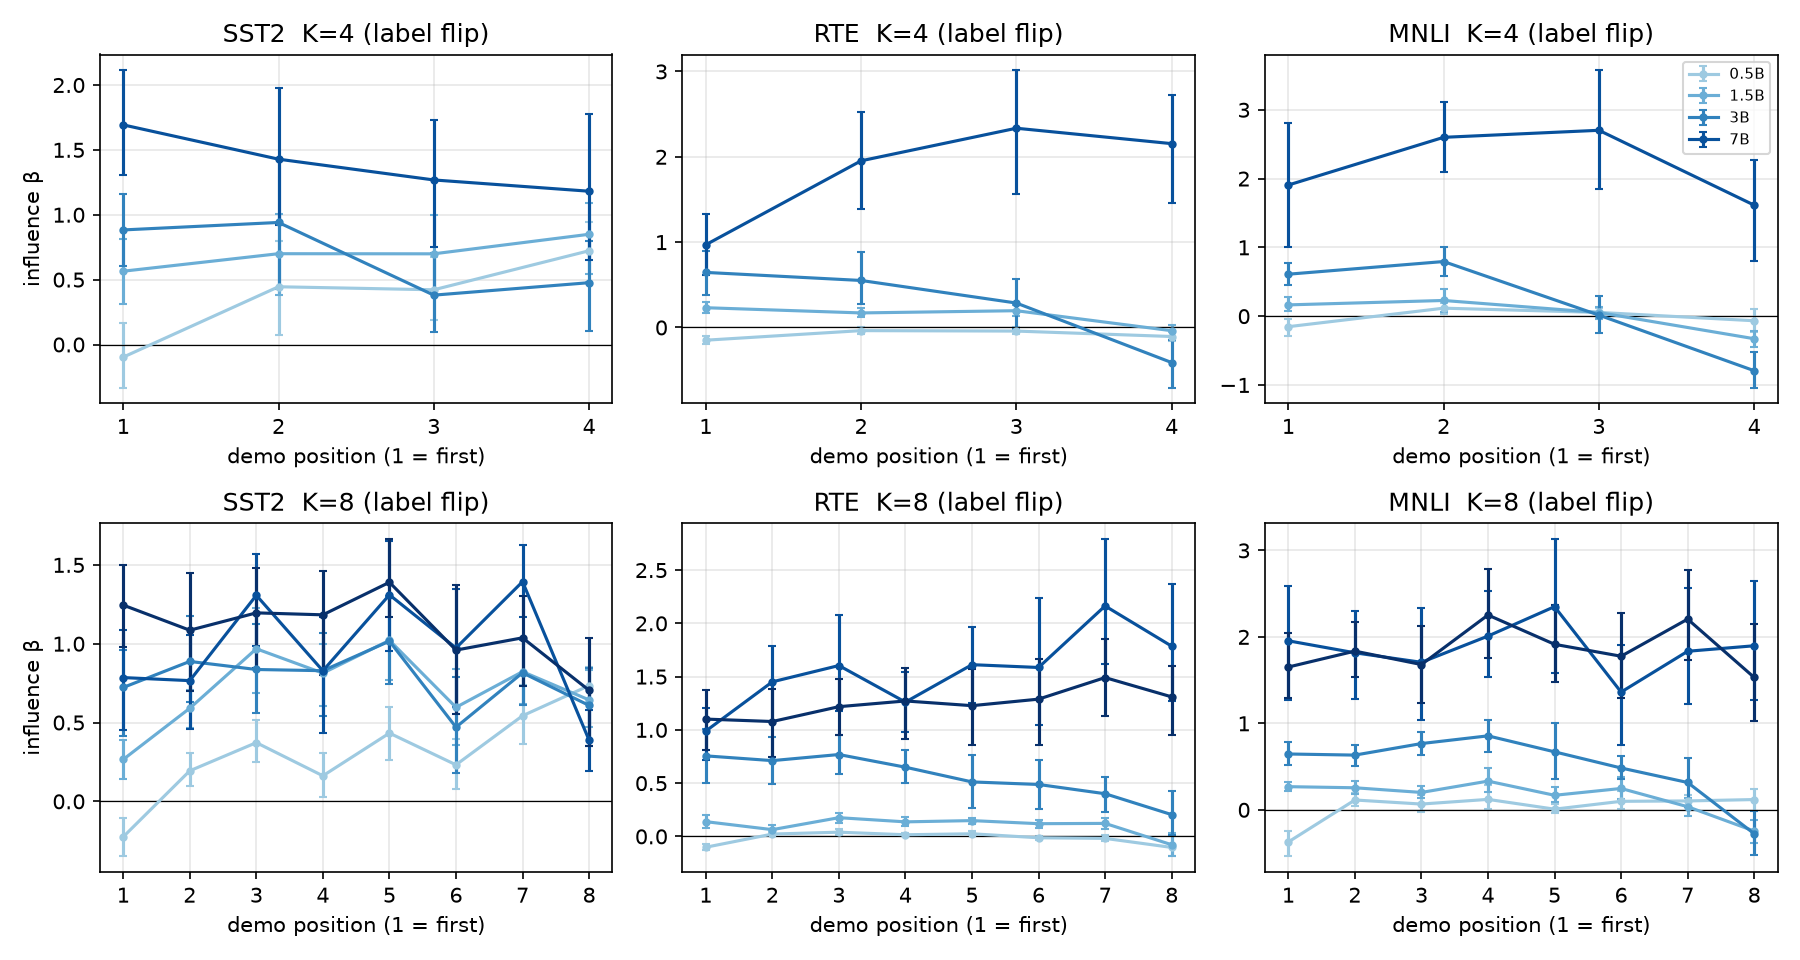
\includegraphics[width=0.95\linewidth]{figures/fig4b_cls_labelflip_influence.png}
\caption{Causal label-flip influence by demonstration position (1 = first) at $K=4$ (top; 0.5B--7B) and $K=8$ (bottom; all sizes, darker = larger). Error bars: 95\% bootstrap CI. Influence rises toward the end only for small models on \sst and for 7B on \rte. On \rte and \mnli, 1.5B and 3B influence turns \emph{negative} at the last position (anti-recency), while 7B and 14B are roughly flat.}
\label{fig:labelflip}
\end{figure}

\begin{table}[t]
\centering
\caption{H2: causal label-flip influence at $K=8$ (nats; increase in $\log P$ of the flipped-to label, averaged over test items, 10 demonstration sets $\times$ 2 orders). The last/first ratio has a 95\% bootstrap CI over demonstration sets. Ratios consistent with H2 (CI above 1 and overlapping 2--3) in \textbf{bold}. ``n/a'': first-position influence is negative or near zero, so the ratio is not meaningful.}
\label{tab:labelflip}
\small
\begin{tabular}{@{}llcccc@{}}
\toprule
Task & Model & Pos.\ 1 & Pos.\ 2--7 (mean) & Pos.\ 8 & Last/first [95\% CI] \\
\midrule
\multirow{5}{*}{\sst} & 0.5B & $-$0.23 & 0.30 & 0.73 & n/a \\
 & 1.5B & 0.27 & 0.80 & 0.64 & \textbf{2.42} [1.83, 3.50] \\
 & 3B & 0.72 & 0.81 & 0.61 & 0.84 [0.52, 1.37] \\
 & 7B & 0.79 & 1.10 & 0.39 & 0.49 [0.25, 0.87] \\
 & 14B & 1.25 & 1.14 & 0.70 & 0.57 [0.29, 0.88] \\
\midrule
\multirow{5}{*}{\rte} & 0.5B & $-$0.10 & 0.01 & $-$0.10 & n/a \\
 & 1.5B & 0.14 & 0.13 & $-$0.08 & $-$0.56 [$-$1.75, 0.23] \\
 & 3B & 0.76 & 0.59 & 0.20 & 0.27 [0.02, 0.52] \\
 & 7B & 0.99 & 1.61 & 1.79 & \textbf{1.81} [1.27, 2.44] \\
 & 14B & 1.10 & 1.26 & 1.31 & 1.19 [0.88, 1.60] \\
\midrule
\multirow{5}{*}{\mnli} & 0.5B & $-$0.37 & 0.08 & 0.12 & n/a \\
 & 1.5B & 0.27 & 0.21 & $-$0.25 & $-$0.92 [$-$1.46, $-$0.46] \\
 & 3B & 0.65 & 0.62 & $-$0.28 & $-$0.43 [$-$0.90, $-$0.03] \\
 & 7B & 1.95 & 1.85 & 1.90 & 0.97 [0.63, 1.52] \\
 & 14B & 1.65 & 1.95 & 1.53 & 0.93 [0.58, 1.37] \\
\bottomrule
\end{tabular}
\end{table}


{\bf Is the last demonstration 2--3$\times$ as influential as the first?}
\Tabref{tab:labelflip} and \figref{fig:labelflip} show that this holds in only 2 of 15 model--task cells at $K=8$: \sst with 1.5B (2.42$\times$, CI [1.83, 3.50]) and \rte with 7B (1.81$\times$ [1.27, 2.44]; 2.22$\times$ [1.71, 2.97] at $K=4$).
For 0.5B on \sst, influence rises steeply toward the end (0.73 nats at the last position), but the first position is slightly negative, so this is recency in shape without a meaningful ratio.
Several cells point the other way: on \sst, 7B (0.49$\times$) and 14B (0.57$\times$) weight \emph{early} demonstrations more.

\para{Anti-recency on NLI.}
For 1.5B and 3B on \rte and \mnli, flipping the \emph{last} demonstration's label lowers the probability of the flipped-to label.
For 3B on \mnli at $K=4$, the last position has influence $-0.79$ nats against $+0.61$ for the first, and at $K=8$ the flip moves predictions 4.2 percentage points \emph{away} from the flipped label.
The effect is concentrated in the final position: influence is flat over earlier positions and then turns negative (\figref{fig:labelflip}).
One possible mechanism is that when the demonstration closest to the test item looks inconsistent, the model contrasts away from it rather than copying it; we did not test this.
Unmanipulated prompts agree: for 3B on \mnli at $K=8$, the prediction matches the label at position 1 for 36.4\% of items and at position 8 for 30.8\% (chance $\approx$33\%); for 14B, 36.8\% \vsx 31.8\%.
Only 0.5B on \sst shows clear recency here (47.8\% \vsx 52.8\%).

The 14B model is roughly position-uniform on \rte and \mnli (ratios 1.19 and 0.93, CIs include 1) and mildly primacy-weighted on \sst.
{\bf H2 is not supported} as a general claim: the direction of the position effect depends on both model and task.
We also fit an observational regression of the label score on the label at each position (\appref{app:details}); its absolute per-position values are poorly identified because they come mostly from label-composition differences between 10--20 demonstration sets, so we treat the causal probe as primary.

\subsection{H3: generation shows recency, not primacy}
\label{sec:h3}

\begin{figure}[t]
\centering
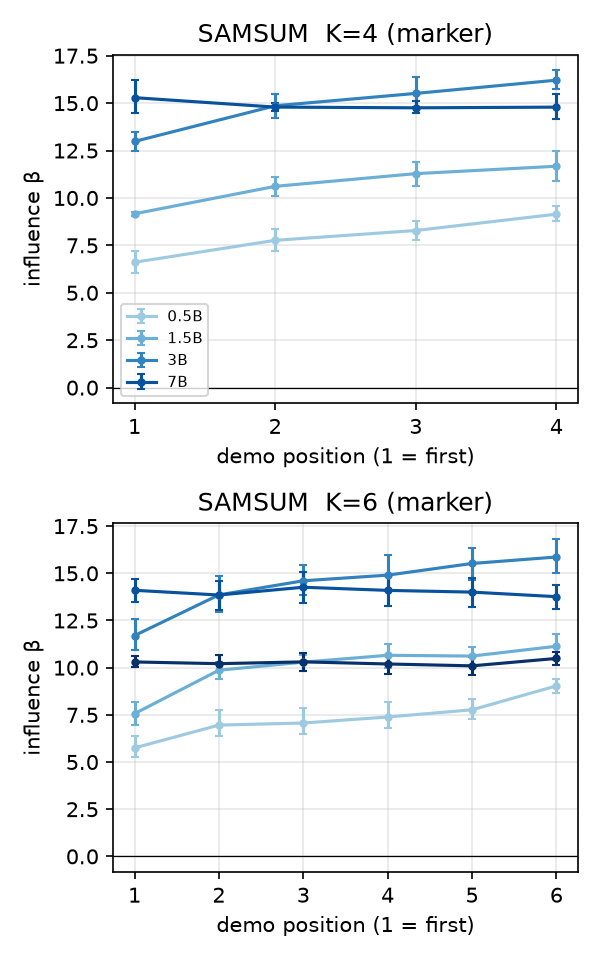
\includegraphics[width=0.3\linewidth]{figures/fig5b_gen_marker_influence.png}
\caption{Style-marker influence on \samsum by demonstration position at $K=4$ (top; 0.5B--7B) and $K=6$ (bottom; all sizes). Error bars: 95\% bootstrap CI. For 0.5B--3B, a marker in a later demonstration is copied more often (recency). For 7B and 14B influence is flat across positions. No model shows the strong primacy predicted by H3.}
\label{fig:marker}
\end{figure}

\begin{table}[t]
\centering
\caption{H3: style-marker influence on \samsum at $K=6$ (nats; increase in $\log P$ that the output begins with ``In short,'' when demonstration $i$'s summary begins with it, relative to no marker). Largest influence per model in \textbf{bold}. H3 predicts a first/last ratio above 1; small models show the opposite.}
\label{tab:marker}
\small
\begin{tabular}{@{}lccccccc@{}}
\toprule
Model & Pos.\ 1 & 2 & 3 & 4 & 5 & 6 & First/last [95\% CI] \\
\midrule
0.5B & 5.75 & 6.96 & 7.07 & 7.39 & 7.77 & \textbf{9.04} & 0.64 [0.59, 0.68] \\
1.5B & 7.56 & 9.87 & 10.29 & 10.66 & 10.61 & \textbf{11.13} & 0.68 [0.62, 0.74] \\
3B & 11.70 & 13.86 & 14.60 & 14.90 & 15.52 & \textbf{15.86} & 0.74 [0.72, 0.75] \\
7B & 14.10 & 13.85 & \textbf{14.26} & 14.10 & 14.00 & 13.76 & 1.02 [1.00, 1.05] \\
14B & 10.30 & 10.21 & 10.31 & 10.20 & 10.10 & \textbf{10.49} & 0.98 [0.95, 1.01] \\
\bottomrule
\end{tabular}
\end{table}


{\bf Does the first demonstration dominate generation?}
\Tabref{tab:marker} and \figref{fig:marker} show that it does not.
For 0.5B, 1.5B and 3B, the influence of a style marker rises monotonically with position: the first/last ratio is 0.64--0.74 at $K=6$ and 0.72--0.80 at $K=4$, with all CIs excluding 1.
At 7B the profile is essentially flat, with a statistically detectable but tiny primacy (first/last 1.02 at $K=6$, 1.03 [1.02, 1.05] at $K=4$, \ie about 3\%).
At 14B it is position-independent (0.98 [0.95, 1.01]).
{\bf H3 is refuted.}
The only primacy we observe (7B) is roughly ten times smaller than the recency seen in the small models (a 2--3\% excess against 20--36\%).
A secondary, non-causal measure, the lexical copying of each demonstration's summary words into the output, is small (under 1.5\% of output words) and noisy, with no consistent primacy.
Because the probe aggregates many paired comparisons on log-probabilities rather than on sampled text, it is less affected by the numerical noise of \secref{sec:reliability}.

\subsection{H5: scale helps on easy classification, not everywhere}
\label{sec:h5}

\begin{figure}[t]
\centering
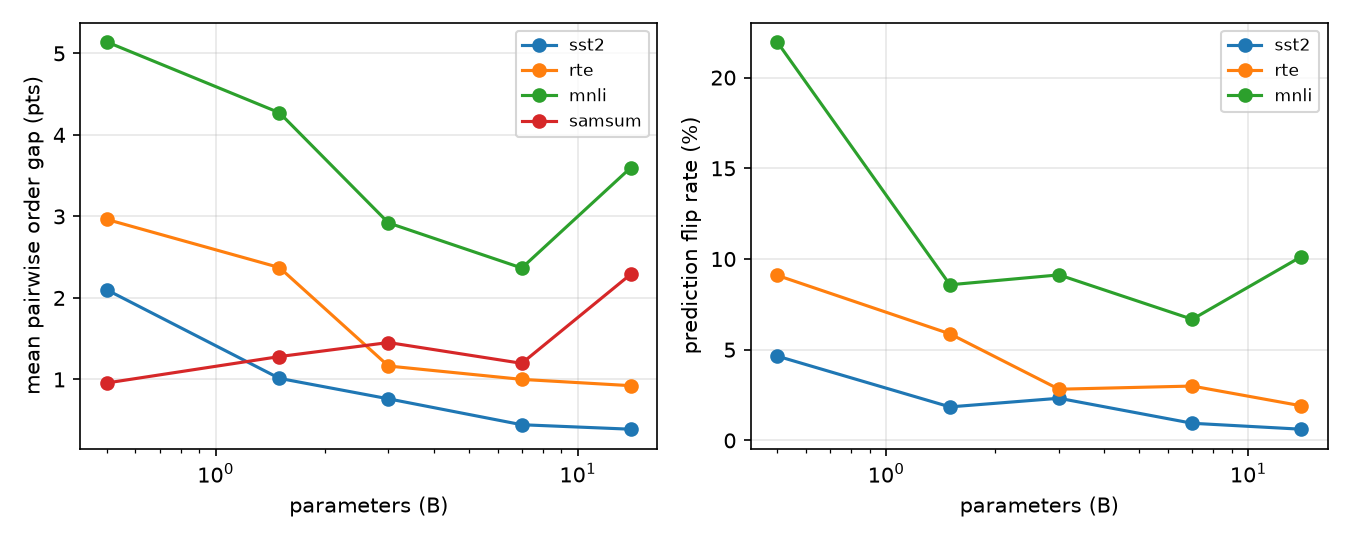
\includegraphics[width=0.8\linewidth]{figures/fig7_size_vs_sensitivity.png}
\caption{Order sensitivity \vsx model size (log scale). \figleft Mean pairwise order gap ($K\geq2$). \figright Prediction flip rate between two orders. Sensitivity falls monotonically with size on \sst and \rte, reaches its minimum at 7B on \mnli, and rises with size on \samsum.}
\label{fig:size}
\end{figure}

\begin{table}[t]
\centering
\caption{H5: order sensitivity by model size ($K\geq2$). \pgap in points; flip rate is the percentage of test predictions that change between two orders. Spearman $\rho$ is over the 5 sizes. Lowest per row in \textbf{bold}.}
\label{tab:size}
\small
\begin{tabular}{@{}llcccccc@{}}
\toprule
Task & Metric & 0.5B & 1.5B & 3B & 7B & 14B & $\rho$ [$p$] \\
\midrule
\sst & \pgap & 2.10 & 1.01 & 0.76 & 0.44 & \textbf{0.39} & $-$1.0 [$<$.001] \\
 & flip rate (\%) & 4.6 & 1.9 & 2.3 & 0.9 & \textbf{0.6} & $-$0.9 [0.04] \\
\rte & \pgap & 2.96 & 2.37 & 1.16 & 1.00 & \textbf{0.92} & $-$1.0 [$<$.001] \\
 & flip rate (\%) & 9.1 & 5.9 & 2.8 & 3.0 & \textbf{1.9} & $-$0.9 [0.04] \\
\mnli & \pgap & 5.14 & 4.27 & 2.92 & \textbf{2.37} & 3.60 & $-$0.7 [0.19] \\
 & flip rate (\%) & 22.0 & 8.6 & 9.1 & \textbf{6.7} & 10.1 & $-$0.3 [0.62] \\
\samsum & \pgap (\rougel) & \textbf{0.96} & 1.28 & 1.45 & 1.20 & 2.29 & $+$0.7 [0.19] \\
\bottomrule
\end{tabular}
\end{table}


\Tabref{tab:size} and \figref{fig:size} show that larger models are less order-sensitive on \sst and \rte: \pgap falls monotonically from 2.10 to 0.39 points on \sst and from 2.96 to 0.92 on \rte (Spearman $\rho=-1$), and flip rates fall from 4.6\% to 0.6\% and from 9.1\% to 1.9\%.
On \mnli the trend is non-monotone: sensitivity is lowest at 7B (\pgap 2.37) and higher again at 14B (3.60).
On \samsum the trend points the other way: 14B is the most order-sensitive model (\pgap 2.29 \vsx 0.96 for 0.5B), and its order effects are the most reproducible (split-half $\rho=0.67$, \tabref{tab:reliability}).
{\bf H5 is supported for \sst and \rte, but not universally.}
With only five sizes from one family, the trend tests are coarse: $\rho=\pm0.7$ is not significant ($p=0.19$).
